\documentclass[../report.tex]{subfiles}

\begin{document}
Trong phần này, chúng ta sẽ xem xét giá trị của các 
tập mờ trong một hệ động học mờ $(F_k^1[0, 1], z_f)$. \\

\noindent Ví dụ 2: Tính toán nguyên lý mở rộng Zadeh bởi $f$ được 
cho bởi tam giá $(0, 0), (1/4, 9/10), (1, 0)$
và tập mờ $A$ được cho bởi $(0, 0), (3/4, 1), (1, 0)$ như trong 
hình \ref{fig:2}.
\begin{figure}[H]
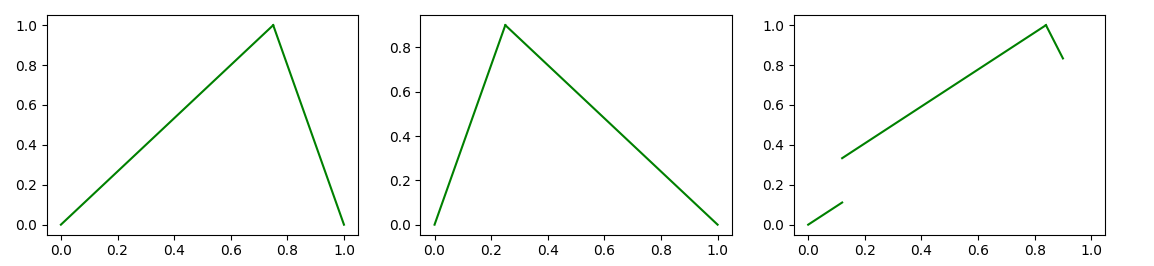
\includegraphics[width=\textwidth]{figures/example2.png}
\caption{Đồ thị của tập mờ $A$, hàm $f$ và $z_f^2(A)$}
\label{fig:2}
\end{figure}

Từ hình trên ta có thể thấy, cho dù với những đồ thị rất đơn giản cho 
các hàm tuyến tính liên tục $f$ và $A$, nguyên lý mở rộng Zadeh 
có thể sinh ra những tập mờ không liên tục, như trong ví dụ trên
$z_f^2(A)$ là không liên tục. Trong hình \ref{fig:3}, 20 giá trị đầu tiên
của quỹ đạo mờ được thể hiện trên đồ thị 3 chiều. 

\begin{figure}[H]
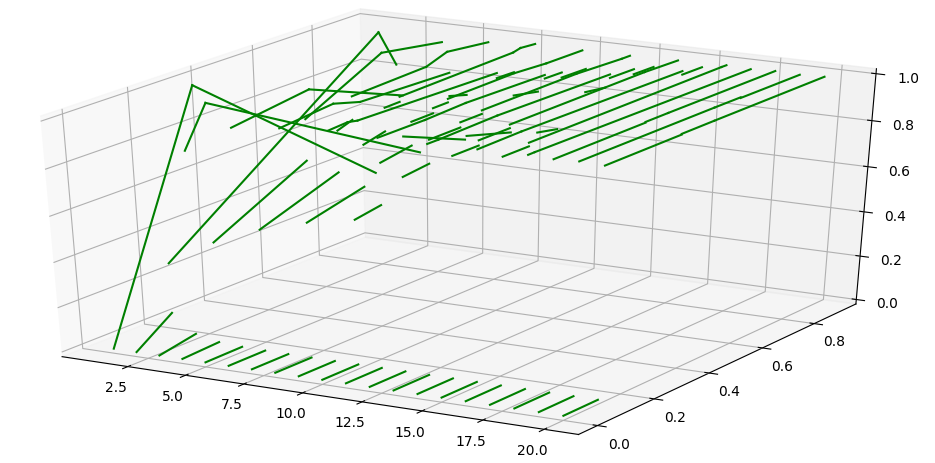
\includegraphics[width=\textwidth]{figures/example2_3d.png}
\caption{20 giá trị đầu tiên của quỹ đạo}
\label{fig:3}
\end{figure}

\end{document}
